%location/filename: tex/ch1.tex
%author: Anders Østevik
%Last edited: 16.12.2015
%#######--Chapter 3--#######
%Content:
%	Interface/Communication between \gls{pc} and FPGA
%	

\documentclass[main.tex]{subfiles}

\usetikzlibrary{arrows,automata}

\begin{document}

\chapter{Serial interface}

In order to connect and control the \gls{cru} with an interface on a user \gls{pc}, a serial communication between the user \gls{pc} and the \gls{fpga} is needed. The purpose of the serial link is mainly to monitor the \gls{gbt} and manipulate the control signals. Because of this, the speed requirements of the link is not a crucial matter. The \gls{fpga} unit used in this thesis (section \ref{sec:cyclone}) has various forms of communication standards readily available. The following sections starts off with an evaluation of the different communication standards available on the \gls{fpga}, and continues with a description of the final implementation of the communication setup.
\\

\section{Readily available standards}
When choosing the serial communication between the \gls{fpga} and the \gls{pc}, factors like physical compatibility, implementation, availability and complexity were taken into consideration. The \gls{fpga} unit has the following communication capabilities readily available: \gls{pci}-express, Ethernet, JTAG UART (through the USB Blaster II), and an SDI-transceiver. The following short sections describe advantages and disadvantages of using one of the systems mentioned above in context with the thesis.\\

The \gls{pci}-express connection requires the \gls{fpga} to be directly mounted on the motherboard of the \gls{pc}, which is in this situation impractical and not necessary for a simple communication link. This option also limits the compatibility with some \gls{fpga} boards and \gls{pc}s that do not have a \gls{pci}-express connection. It does, however, enable for very fast data transmission and removes potential noise generated by using external cabling. \\

The ethernet connection is integrated in most \gls{fpga} boards, but requires layers of protocols in order to communicate. This might be unnecessarily complex for a simple communication link. The upside is that an ethernet connection offers long distances between the \gls{pc} and FPGA, either through networking or long cabling. Using ethernet for communication only requires a known IP-address between the devices for connection and transmission, no additional drivers. \\

The \acrshort{sdi}-transceiver is meant for audio/video transmission and uses \acrshort{bnc}-connectors for this task. It therefore requires special audio/video equipment on the \gls{pc} side for connection and transmission, which is not necessary for a simple communication link.\\

Serial communication through the Altera JTAG UART IP is possible through the only \acrshort{usb}-connection on the board; the USB Blaster II, which is used to program the \gls{fpga}. This requires the implementation of the Nios II soft processor. A soft processor is a microprocessor implemented into the \gls{fpga} with the help of logic synthesis only. While it is also possible to use a \gls{hps}, only a few \gls{fpga}-boards (SoC-boards) comes with one implemented. There is no support for \gls{hps} on the \gls{fpga} board that is used in this thesis. Using this approach limits the user to send and receive characters through a dedicated System Console, offered by Altera \cite{altera_terminals14}. A Nios II-extension for the Eclipse \acrshort{ide} in combination with the C programming language is commonly used to program the soft processor.\\

While attempts were made to implement the Nios II and write a simple send- and receive routine in C, this method for communication seemed overly complex for the purpose for manipulation of the \gls{gbt} control signals. In addition, there was also issues with debugging and the project was abandoned.\footnote{The most serious debugging issue using Eclipse Nios II \acrshort{ide} was that the compiler continued displaying errors after the errors were corrected. Even after the actual bugged function or line of code were deleted completely, the compiler would point to the empty void of which the function or line of code previously were, and call the same error as before it was deleted. This made the dedicated Nios II compiler unreliable, and the code impossible to debug.} Not only did this approach make it a whole lot more complicated, but it was also more error prone and permits the use of user defined software for communication with the \gls{fpga}.

\section{User defined communication}

In addition to the communication standards described above, which in turn requires specific cable- and socket types for connection, it is possible to connect the transmit and receive signals directly to the \gls{fpga} pinout. The only requirement is that the given \gls{fpga} has unoccupied transmitter and receiver signal pins available for the user; either through a HSMC-port (with the help of an additional GPIO-extension board), or through a prototype area or header.\footnote{The user has to assign the available pins to the associated transmitter and receive signals in the \textit{Pin Planner} program, as part of Quartus II suite.}\\

The \gls{fpga} unit that is used in this thesis has no dedicated prototyping area for external signal connection. It instead comes with an GPIO-extension board that connects to one of the two on-board HSMC-ports.\footnote{By using both the HSMC-ports on the \gls{fpga}, the GPIO-\gls{pcb} could not fit properly side-by-side with the \acrshort{hsmc}-to-\acrshort{vldb} \acrshort{pcb} (section \ref{chap:pcb}) because the latter \gls{pcb} is a bit to wide.} However, if removing the on-mounted LCD-display, it is possible to use the exposed header for signaling. The header (J10 in the board schematic) is connected to a transmitter- and receiver pair (both running on 5 volts), several 5 volt output pins and a ground pin. Using the transmitter- and receiver pair from the available header, it is possible to implement a type of asynchronous serial protocol into the \gls{fpga}.\\

The communication protocols described above are summed up in the table below.

Common to all communication systems considered is that they are all duplex systems, which simply means two connected devices that can both transmit and receive signals. While \textit{full-duplex} enables both devices to transmit and receive simultaneously (like a telephone), \textit{half-duplex} only enables one device to transmit at a time (like a walkie-talkie). Common to both the duplex systems is that they have two communication channels. 

\section{Choosing communication protocol}
Perhaps the most well-known serial communication standard is the \gls{rs232} standard. It supports both synchronous and asynchronous transmission, and only requires a single transmit- and receiver pair (if excluding the data control signals). It is compatible over a wide range of voltage levels, and can be connected directly to the serial port of a \gls{pc} or through a \gls{usbrs}. \\

For simplicity, the \acrshort{rs232}-standard was therefore chosen as the communication protocol. A simple \gls{uart} with a byte-decoder was implemented on the \gls{fpga}-side. On the \gls{pc} side, a dedicated C-program was written with the help of the serial library \textit{Termios} to send and receive bytes to and from the \gls{fpga}.  A \gls{usbrs} was used to connect the \gls{fpga} to the \gls{pc}. 

\chapter{Implementing a serial interface into the FPGA}

\section{Transmission protocol: RS-232}

\gls{rs232} standard is a transmission protocol for full duplex, serial transmitting and receiving of data. The standard defines electrical characteristics and timing of signals, the "meaning" of the signal, and also physical size and pin-out for connectors.
For communications to work properly, both the \gls{dte} (the \gls{pc}) and  the \gls{dce} (in this case, the \gls{fpga}) needs to agree on the same data-packet setting, i.e the baud rate, the number of data bits, any additional parity bit and the number of stop bits.\\

A typical \gls{rs232} data-packet consists of a start bit, followed by 5, 7 or 8 data bits; 1 parity bit, for error checking; and 1 or 2 stop bits, indicating that the transmission is done. The start bit is typically a logical low and the stop bit(s) high (this can be system dependent). The transmission line remains high until the start bit pulls it down low, and the data transfer begins until the stop bit is reached. The line is then kept high until a new start bit pulls it low again for a new byte to be transfered. Data-packets are often described in the form: $115200-8-N-1$, which simply means $115200~ \bit\per\second$, $8~ data~ bits$, $No~ parity$ and $1~ stop~ bit$. Figure \ref{fig:rs232} demonstrates a typical \gls{rs232} signal.\\

\begin{figure}[!h]
\begin{center}
\begin{tikzpicture}

\timing [
yscale=2.0,
timing/wscale=3.0,
timing/inline 
node/.style={below left, font=\sffamily\scriptsize}
] at (0,0)
{
H N {$Idle$}
L N {$Start$} 
D {$D_0$} 
D {$D_1$} 
D {$D_2$} 
D {$D_3$} 
D {$D_4$} 
D {$D_5$} 
D {$D_6$}  
D {$D_7$} 
D {$Parity$} 
H N{$Stop$}
%L H N[xscale=.8]{ACK} 
H N{$Idle$}
};

\end{tikzpicture}

\caption{Example of an \gls{rs232} signal with 8 data bits, 1 parity bit (ODD or EVEN) and 1 stop bit.}
\label{fig:rs232}

\end{center}
\end{figure}


\section{HDL on the FPGA side}

When designing an \gls{uart}, it is possible to use an Altera IP which sets up an \gls{uart} for you. However, for learning purposes, this thesis uses an \gls{uart} that is  

Simply put, an \gls{uart} is a circuit that transmits and receives parallel data through a serial line \cite{chu08}.

The \gls{uart}-design is divided into five parts:\\
- A Receiver that receives the serial data and reassembles it into parallel data.\\
- A Transmitter that sends parallel data bit by bit out the serial line.\\
- A Baud Rate Generator that generates the right amount of ticks relative to the baud rate and global clock.\\
- Two \gls{fifo}-registers connected to the transmitter and receiver to shift the data in or out.\\

The following sections gives a brief description of each of the parts described above. \\
The design is based on the \gls{uart} design by Pong P. Chu, found in chapter 7 from his book \textit{FPGA Prototyping By VHDL Examples}  \cite{chu08}, with the exception of the Baud Rate Generator, which was borrowed from the \textit{Uart2Bus} \acrshort{vhdl}-design by Arild Velure. The end result forms a \gls{uart} that receives and transmits $115200-8-N-1$ \gls{rs232} data-packets.

\subsection{UART oversampling and the Baud Rate Generator}

To obtain an accurate sampling of the received signal, an asynchronous system like the \gls{uart} uses what is referred to as oversampling. \\
With a typical rate of 16 times the baud rate, the receiver listens for the line to go from idle to the first start bit. When pulled low or high (depending on the system), a counter starts counting from 0 to 7. When the counter reaches 7, the received signal is roughly in the middle of the start bit. By sampling the bit in the middle of its time frame, the receiver avoids the noise and ringing that are generated whenever a serial bit changes \cite{rapid08}. When in the middle of the start bit, the counter needs to tick 16 times before it reaches the middle of the first data bit, the \gls{lsb}. The \gls{lsb} can now be sampled, and the procedure is repeated $N - 1$ times until reaching the last data bit, the \acrshort{msb}. If there is a parity bit, the same procedure is repeated one more time to retrieve it. After retrieving all the data bits, the same procedure is used one last time to sample the M stop bits at the end of the signal. After this, the line is held high until a new start bit arrives. 

%\mdfdefinestyle{mystyle}{rightmargin=90pt, linecolor=darkgray}

\begin{figure}[!htp]
\begin{center}
%\begin{minipage}[!h]{0.85\linewidth}  %Needed this to lign the figures up properly
%\begin{mdframed}%[style=mystyle]
\begin{tikztimingtable}[%
    timing/dslope=0.5,
    timing/.style={x=1ex,y=4ex},
    x=4ex,
    timing/rowdist=5ex,
    %timing/coldist=2ex,
    xscale=0.8,yscale=0.7, % scale diagrams
    timing/name/.style={font=\sffamily\scriptsize}
    ]
\\
Data      & 14h 28l 28d{$d_0$} 28d{$d_1$} 28d{$d_2$} \\%16d{$d_3$} 16d{$d_4$} 16d{$d_5$} 16d{$d_6$} 16d{$d_7$} 16d{$stop$}H \\
Sample ticks        & h 125{c}\\
\\
%\vspace{20pt}
%AD   & 2u 1D{addr} 1U{} 1D{$d_1$} D{$d_1 '$} D{$d_2$} 2D{$d_3$} U \\
%C/BE & 2u 1D{0010} 6D{BE\#} U  \\
%IRDY      & UU 4L HLH \\
%TRDY       & UU HLH 3L H \\
%DEVSEL     & 2U 6L H\\
\extracode
\begin{pgfonlayer}{background}
\begin{scope}[semithick]
\vertlines[darkgray, dotted]{1.75, 3.5}
\vertlines[darkgray,dotted]{7.0, 10.5,...,14}
  
  \draw[<->] (1.75,-10) -- (3.5,-10) node [midway,below] {\scriptsize 8 cycles};
  \draw[<->] (3.5,-10) -- (7.0,-10) node [midway,below] {\scriptsize 16 cycles};
    \draw[<->] (7.0,-10) -- (10.5,-10) node [midway,below] {\scriptsize 16 cycles};
      \draw[<->] (10.5,-10) -- (14.0,-10) node [midway,below] {\scriptsize 16 cycles};

  \draw[<-] (3.5, 1) -- (3.5,2) node [midway,above] {\scriptsize Middle};
 \draw[] (3.5, -2.6) -- (3.5,-2.6) node [midway,above] {\tiny Start bit};
  \draw[<-] (7, 1) -- (7,2) node [midway,above] {\scriptsize Sample LSB};
  \draw[<-] (10.5, 1) -- (10.5,2) node [midway,above] {\scriptsize Sample d1};
  \draw[<-] (14, 1) -- (14,2) node [midway,above] {\scriptsize Sample d2};

\end{scope}
\end{pgfonlayer}
\end{tikztimingtable}
%\end{mdframed}
\caption{\gls{uart} receive synchronisation and data sampling points with 16 times the sampling rate.}
\label{fig:uartsample}
%\end{minipage}
\end{center}

\end{figure}


To achieve a sampling rate of 16 times the baud rate, a Baud Rate Generator module is implemented into the design. The module generates a one-clock-cycle tick once every $\frac{clock}{16 \times baud\ rate}$ clock cycles. For a baud rate of $115200\ \bit\per\second$ and a clock of $50\ \mega\hertz$, there must be a one-clock-cycle tick once every $27$ clock cycle. This is achieved by counting in certain steps given by the formula below:

\begin{equation}
Baud\ frequency = \frac{16 \times baud\ rate}{GCD(clock, 16 \times baud\ rate)}
\end{equation}

, where baud frequency is the count steps, GCD is the greatest common divisor between the global clock and the baud rate times 16 \cite{velure10}. \\
For a baud rate of $115200\ \bit\per\second$ and a clock of $50\ \mega\hertz$, the counter must count in steps of $576$ per clock cycle. 

Once the counter reaches a given baud limit, the counter resets and the tick-signal is pulled high. After one clock cycle, the tick-signal is pulled low and the counter starts to count upwards again. The baud limit is given by:

\begin{equation}
Baud\ limit= \frac{clock}{GCD(clock, 16 \times baud\ rate)} - baud\ frequency
\end{equation}

, where clock is the global clock of the system and GCD is the greatest common divisor between the global clock and the baud rate times 16 \cite{velure10}. \\
For a baud rate of $115200\ \bit\per\second$ and a clock of $50\ \mega\hertz$, the counter must count in steps of $576$ up to the baud limit of $15049$, before pulling the tick-signal high and start over again. 

\subsection{UART Receiver}
The receiver is essentially a finite state machine, divided into four states: the idle-, start-, data- and stop state. It uses the Start and Stop bits to reset the state machine in an attempt to synchronize the clock phase to the incoming signal. For this, the receiver contains three registers: the s- and  n registers for counting, and a b register for data storing. The s-register keeps track of the sample ticks and n-register the number of data bits sampled.
There are two constants defined for the receiver: the $DBIT$ constant, which indicates the number of data bits; and the $SB\_TICK$ constant, which indicates how many ticks that is required for the stop bit(s) (16 ticks for 1 stop bit). 

\begin{figure}[!htp]
\begin{center}
%\usetikzlibrary{arrows,automata}
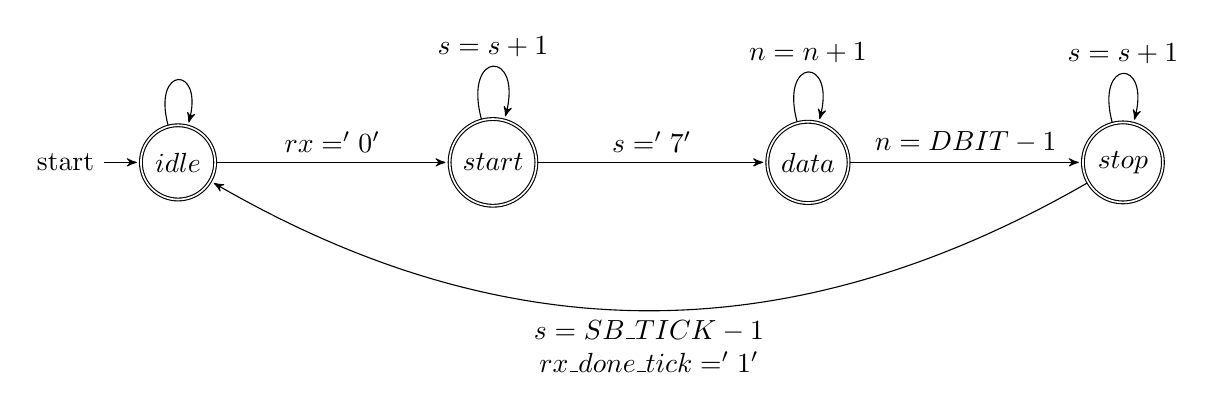
\begin{tikzpicture}[>=stealth',shorten >=1pt,auto,node distance=4cm]
  \node[initial,state,accepting] (idle)      {$idle$};
  \node[state,accepting]         (start) [right of=idle]  {$start$};
  \node[state,accepting]         (data) [right of=start] {$data$};
  \node[state,accepting]         (stop) [right of=data] {$stop$};
 
  %\path[->]          (S)  edge [loop above] node {a} (idle);
  \path[->]          (idle)  edge [loop above] node {} (idle);
  \path[->]           (idle)  edge              node {$rx = '0'$} (start);
  \path[->]          (start)  edge [loop above] node {$s = s+1$} (start);
  \path[->] (start) edge             node {$s = '7'$} (data);
  \path [->]             (data) edge [loop above] node {$n = n+1$} (data);
  \path[->] (data) edge             node {$n = DBIT-1$} (stop);
  \path [->]             (stop) edge [loop above] node {$s = s+1$} (stop)
             edge [bend left]  node[align=center] {
             $s = SB\_TICK-1$ \\ $rx\_done\_tick = '1'$
             } (idle);
\end{tikzpicture}
\caption{\gls{uart} receiver state machine.}
\label{fig:uartrx}
\end{center}
\end{figure}

Starting with the idle state: given that there is not already a signal being received and sampled (i.e $rx\_done\_tick = '1'$), the receiver waits for the rx-signal to go low (i.e detecting a start signal). The s-register then resets and the state machine goes to the next state: the start state. \\

When in the start state, the ticks generated by the baud rate generator clocks the s-registers and waits for it to count up to 7 (i.e in the middle of the start-bit). It then resets the s- and n-registers and sets the next state to the data state. Since the received signal so far is the middle of the start bit, the s-register must count up to 15  before reaching the middle of the data bit so that the b-register can sample the data. Each time the s-register reaches 15, the b-register shifts in the rx by 1 bit while the n-register increments by 1, keeping track of the bit width. When the n-register reaches a count equal to the $DBIT$ constant minus 1, the transmission is at its end, and the state machine shift to the last state: the stop state. \\

The stop state uses the sample ticks in conjunction with the s-register to count the stop bit(s) duration by using the $SB\_TICK-1$ as the upper count limit. When done, the  $rx\_done\_tick$ signal is set to 1 and the state machine shifts back to the idle state. We have now successfully received a serially  transmitted byte. %The state machine is shown in figure \ref{fig:uartrx}. 

\subsection{UART Transmitter}
The \gls{uart} transmitter has a similar design to that of the receiver; it uses the same state machine structure, but for the purpose of shifting out data. In addition to the s-, n-, and b-registers used for counting, the transmitter contains a din-register for input parallel data and a $1~\bit$ tx-register for shifting out the data. Connected to the tx-register is a tx output signal. To prevent multiple clocks, the baud rate generator is also used to clock the transmitter. For the transmitter to be properly synchronized with the receiver, it instead uses the counter registers to slow down the operation 16 times. This is because there is no oversampling involved in transmitting a signal.\\

\begin{figure}[!htp]
\begin{center}
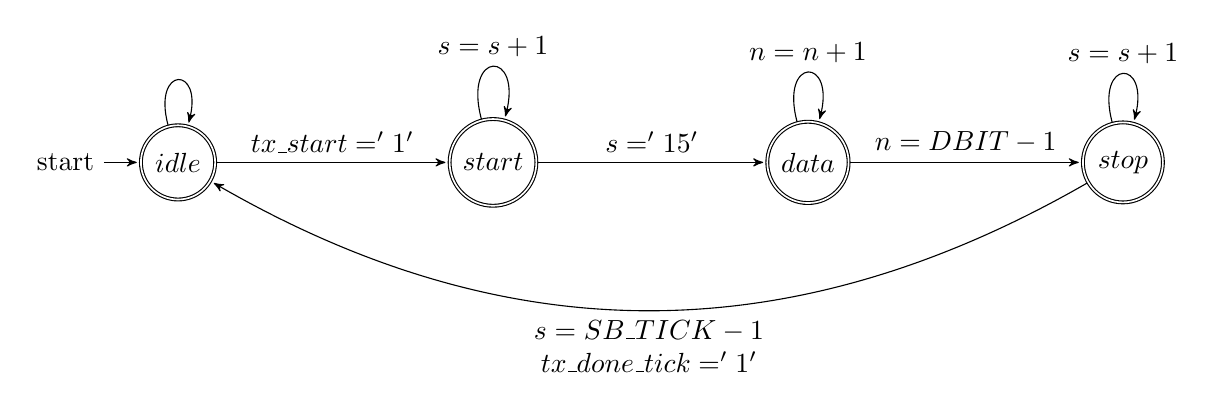
\begin{tikzpicture}[>=stealth',shorten >=1pt,auto,node distance=4cm]
  \node[initial,state,accepting] (idle)      {$idle$};
  \node[state,accepting]         (start) [right of=idle]  {$start$};
  \node[state,accepting]         (data) [right of=start] {$data$};
  \node[state,accepting]         (stop) [right of=data] {$stop$};
 
  %\path[->]          (S)  edge [loop above] node {a} (idle);
  \path[->]          (idle)  edge [loop above] node {} (idle);
  \path[->]           (idle)  edge              node {$tx\_start = '1'$} (start);
  \path[->]          (start)  edge [loop above] node {$s = s+1$} (start);
  \path[->] (start) edge             node {$s = '15'$} (data);
  \path [->]             (data) edge [loop above] node {$n = n+1$} (data);
  \path[->] (data) edge             node {$n = DBIT-1$} (stop);
  \path [->]             (stop) edge [loop above] node {$s = s+1$} (stop)
             edge [bend left]  node[align=center] {
             $s = SB\_TICK-1$ \\ $tx\_done\_tick = '1'$
             } (idle);
\end{tikzpicture}
\caption{\gls{uart} transmitter state machine, similar to that of the receiver.}
\label{fig:uarttx}
\end{center}
\end{figure}

When in the idle state, the tx-register is held high for idle line and the b-register is connected to the din register for data input. The state machine remains in the idle state until the $tx\_start$ signal changes from low to high. It then shift to the start state to begin the transmission of the data stored in the b-register. \\

When in the start state, the tx-register is held low for the start bit to be transmitted out. When the s-register reached the count of 15, the start bit is transmitted and the state machine shifts to the data state to further transmit the actual data bits.\\

When in the data state, the tx-register is set to the first bit of the b-register, while the b-register shift its data using a simple right shift operation every 16 clock ticks (s-register reaches 15). To keep track of how many data bits that have been transmitted, the n-register increments by 1 at the same rate as the b-register shifts the data (same as for the receiver). When reaching $DBIT-1$, the data bits is finished transmitting out and the state machine shifts to the stop state.\\

When in the stop state, the tx-register is held high indicating a stop bit is being transmitted. When the s-register reaches a count equal $SBIT - 1$, the stop bits are finished transmitting. The $tx\_done\_tick$ signal is set to high and the state machine shifts back to the idle state, ready to transmit the next data byte.


\subsection{FIFO buffers}
The $rx\_empty$ signal remains low until as long as there are bytes stored in the \gls{fifo}.  

\subsection{UART decoder}
The \gls{uart} decoder is a state machine connected to the other end of the \gls{uart} receiver- and transmitter \glspl{fifo}. It reads out the received bytes and does tasks according to the order and value of the bytes. Starting at the idle state, the decoder waits for a request byte from the fifo followed by an address byte. The request byte can for instance be a read or a write. The following small sections describes the different decoder states. \\

\subsubsection{Idle state}
Being initially in the idle state, the decoder is triggered by the $rx\_empty$ signal coming from the rx-fifo, which is held low if there is at least one byte stored in the rx-fifo. If $rx\_empty$ is low, the decoder sends a read signal ($rd\_uart$), telling the rx-fifo to place the next in-line byte on the read-bus (rdata), and in the same delta-time assigns the read-bus to a new register ($b\_reg(0)$) for temporary storage. The decoder then goes to a read state.\\

\subsubsection{Read1 state}
 In the read1 state, the first temporary stored byte is analyzed. The byte must have a value that is equal to one of three predefined constants, called requests (See $uart\_gbt\_pkg.vhdl$). This first byte is interpreted as a read- or write-request, sent from the client \gls{pc} through the serial connection. If the request-byte is equal to a "read" request, a "write 0" request or a "write 1" request, the decoder goes on to a wait state. If the byte is not a request-value, the state machine returns back to idle and reset the registers.\\

\subsubsection{Wait1 state}
  In the wait1 state, the decoder waits for the next arriving byte after the first one. The wait state does the same as the idle state, i.e waits for $rx\_empty$ to become low before reading out the next byte from the rx-fifo. To prevent the state machine from getting stuck in the wait state (if an address byte does not arrive in time), an additional count-register, triggered by the baud generator ticks, counts up to a predefined value, $C\_TIMEOUT$. $C\_TIMEOUT$ is defined to be a reasonable larger value than the pre-estimated time it takes for the next byte to arrive, i.e $16 ~ticks\per\bit \times 10 ~bits$. If $rx\_empty$ is not triggered low before the count-register has finished counting, the state machine resets to idle. If the next byte arrives before timeout, the decoder stores it and goes to the final state.\\

  \subsubsection{Read2 state}
  In the read2 state, the value of the first byte, the request-byte, decides if the decoder should perform a read or a write operation on the gbt-register. The value of the last received byte is treated as an address to the data of the gbt-register the client wants to read or write to.  

\section{Software on the PC side}
The program is based on 
To access the serial port on the \gls{pc}, the 


\end{document}